\documentclass[12pt]{article}
\usepackage{mathpazo}
\usepackage{hyperref}
\usepackage{enumitem}
\usepackage{graphicx}
\usepackage{xcolor}
\usepackage{textcomp}
\usepackage{booktabs}
\usepackage{longtable}
\usepackage{soul}
\setuldepth{model}
\usepackage{everysel}

% This is to fix full justification for \texttt{}. Credit:
% https://texblog.net/latex-archive/plaintex/full-justification-with-typewriter-font/
\ttfamily
\fontdimen2\font=0.4em% interword space
\fontdimen3\font=0.2em% interword stretch
\fontdimen4\font=0.1em% interword shrink
\fontdimen7\font=0.1em% extra space

% Credit: Stefan Kottwitz, https://latex.org/forum/viewtopic.php?t=13230
\newcommand*{\Biggg}[1]{\vcenter{\hbox{\scalebox{3}{\ensuremath#1}}}}
\newcommand*{\Bigggg}[1]{\vcenter{\hbox{\scalebox{8}{\ensuremath#1}}}}

\usepackage[top=2.54cm, bottom=2.54cm, left=2.54cm, right=2.54cm]{geometry}
\usepackage{tikz}
\usetikzlibrary{fit}
\usetikzlibrary{calc}
\usetikzlibrary{matrix}
\usetikzlibrary{calligraphy}
\usetikzlibrary{arrows.meta}
\usetikzlibrary{shapes.misc}
\usetikzlibrary{intersections}
\usetikzlibrary{shapes,arrows}
\usetikzlibrary{shapes.multipart}
\usetikzlibrary{shapes.geometric}
\usetikzlibrary{shadows,shadings}
\usetikzlibrary{tikzmark,positioning}
\usetikzlibrary{decorations.markings}
\usetikzlibrary{decorations.pathreplacing}

\tikzstyle{stochnode}=[black, draw=black, line width=1.5pt, shape=circle, fill=white, minimum size=8mm, inner sep=3pt]

\tikzstyle{detnode}=[black, draw=black, line width=1.5pt, densely dashed, shape=circle, fill=white, minimum size=8mm, inner sep=3pt]

\tikzstyle{constnode}=[black, draw=black, line width=1.5pt, shape=regular polygon, regular polygon sides=4, fill=white, minimum size=8mm, inner sep=1pt, align=center]

\tikzstyle{clampnode}=[black, draw=black, line width=1.5pt, shape=circle, fill=black!20!white, minimum size=8mm, inner sep=3pt]

\begin{document}
\frenchspacing

\begin{center}
{\Large \textbf{Lab 6. Bayesian inference using RevBayes}} \\[0.5cm]
{\large Due Wednesday, November 9, 2022 at 3 pm}
\end{center}

\vspace{1cm}

\noindent This week, we're going to do something completely different and take a break from phylogenetics. We do this to familiarize ourselves with yet another piece of software called RevBayes (named after Reverend Bayes, of Bayes' rule fame), which is a little bit more involved than what we've used so far and which we will stick with for the rest of the course. Our goal today is to learn how to craft our own analyses from the building blocks RevBayes provides us with, and make sure we understand every step along the way. \\

\hrule

\section*{Software}

Unlike IQ-TREE and similar programs, which were designed to do one specific thing (maximum likelihood phylogenetic inference), RevBayes tries to be a one-stop shop for all things Bayesian. Another important difference is the amount of freedom RevBayes affords its users. Our interaction with PAUP* and IQ-TREE took the form of choosing between pre-selected options and adjusting a few toggles that were hardcoded into the software. In contrast, RevBayes provides the user with a wide variety of building blocks that can be mixed and matched in a myriad of different ways, some of which were not foreseen even by its developers. The flip side of this freedom is that we really have to understand what we're doing, since compared to PAUP* or IQ-TREE, it's much harder to treat RevBayes as a black box that gobbles up data on one end and spits out a tree on the other. This tutorial is therefore largely designed to help you become an informed RevBayes user. \\

\noindent As it turns out, RevBayes is more similar to \textsf{R} than to any of the other programs we've worked with so far, in that it is both a piece of software and a language. In the case of RevBayes, the underlying language is called Rev, and it should look somewhat familiar, since it's designed to feel a lot like \textsf{R} -- though with a few important differences we'll go into later. As with \textsf{R}, we can interact with RevBayes either interactively or by executing scripts. In this lab, we'll take it easy and use the interactive mode, building up our analyses step by step. However, just like before, you are strongly encouraged to keep a record of all the commands you've entered into RevBayes -- and if you save those in a plain-text file with a \texttt{.Rev} extension, that's going to be your Rev script. \\

\noindent RevBayes is available for free on all platforms (Windows, macOS, Linux) and can be downloaded from \url{https://revbayes.github.io/download}. There is no single comprehensive manual for it, but you can access its documentation at \url{https://revbayes.github.io/documentation}, and there is a whole bunch of excellent tutorials available at \url{https://revbayes.github.io/tutorials}. There is even a series of video tutorials available from YouTube: \url{https://www.youtube.com/channel/UCp46ywpZ5edFHuMG5CxVkig}. RevBayes developers also like to organize workshops and teach RevBayes in their own classes (\ldots like we're doing right now!), and with a little bit of googling, you can find very informative PowerPoint slides they've created for these occasions. \\

\noindent Although RevBayes is very powerful and perfectly capable of processing and summarizing its own output, it often helps to inspect its results visually. To do this, we will use another program called Tracer, which you can download from \url{https://github.com/beast-dev/tracer/releases/tag/v1.7.2}. Tracer requires Java (version 1.8 or higher), so you'll need to install the latter as well if you don't already have it.

\section*{Getting started}

Open a terminal (macOS, Linux) / command-line (Windows) window and navigate to the directory with your RevBayes executable. As before, you can use the command \texttt{cd} (\ul{c}hange \ul{d}irectory) to move between directories. On macOS and Linux, you can also use the command \texttt{ls} to \ul{l}i\ul{s}t the contents of your current directory; on Windows, the corresponding command is \texttt{dir}. You can use these to verify that the executable -- called \texttt{rb} -- is indeed present in the place where you're looking for it. \\

\noindent Next, let's launch RevBayes by typing \texttt{./rb} (macOS, Linux) or just \texttt{rb} (Windows) into the command line. This will start the program and give you a command prompt (the \texttt{>} character) indicating that RevBayes is waiting for your further actions. For me, this is what it looks like: \\

\begin{center}
\noindent\includegraphics[width=0.8\textwidth]{revbayes-prompt.png}
\end{center}

\noindent As we learned above, RevBayes is less monomaniacally obsessed with phylogenetics than other programs we've worked with. For starters, we can just use it as a calculator. Each of the lines below will get automatically executed once we hit Enter / Return: \\

\indent \texttt{> 3 + 3} \\
\indent \texttt{\ \ \ 6} \\
\indent \texttt{> 10 - 5} \\
\indent \texttt{\ \ \ 5} \\
\indent \texttt{> 4 * 4} \\
\indent \texttt{\ \ \ 16} \\
\indent \texttt{> 2\^{}3} \\
\indent \texttt{\ \ \ 8} \\

\noindent We can take it one step further and evaluate functions, just like we did in \textsf{R}: \\

\indent \texttt{> exp(5)} \\
\indent \texttt{\ \ \ 148.4132} \\
\indent \texttt{> sqrt(16)} \\
\indent \texttt{\ \ \ 4} \\

\noindent Note that RevBayes is (once again just like \textsf{R}) case-sensitive, so it will complain and refuse to co-operate if you attempt the following function call: \\

\indent \texttt{> Exp(5)} \\
\indent \texttt{\ \ \ Error: \ \ \ \ \ \ No function named \textquotesingle Exp\textquotesingle} \\

\noindent It's not just numbers we can play with -- strings of text work, too: \\

\indent \texttt{> print("Hello world!")} \\
\indent \texttt{Hello world!} \\

\noindent We can even use constructs we know from other programming languages, such as \texttt{for} loops to iterate over a range of values. In the example below, the parentheses specify an iterator \texttt{i} ranging from 1 to 5. For each value in this range, we execute the code located inside the curly braces: \\

\indent \texttt{> for(i in 1:5) \{} \\
\indent \texttt{+\ \ \ \ print(i+" is my favorite number!")} \\
\indent \texttt{+ \}} \\
\indent \texttt{1 is my favorite number!} \\
\indent \texttt{2 is my favorite number!} \\
\indent \texttt{3 is my favorite number!} \\
\indent \texttt{4 is my favorite number!} \\
\indent \texttt{5 is my favorite number!} \\

\noindent (Note how the prompt symbol changed from \texttt{>} to \texttt{+} after we ended the first line with a left curly brace. This means that RevBayes expects more input to follow, and won't start executing the code we've typed until we close the loop with a matching right curly brace.)

\section*{Constant, deterministic, and stochastic variables}

Just like in \textsf{R}, we can \textit{assign values to variables} in RevBayes, but there is an important difference: RevBayes distinguishes between three different kinds of variables called \textit{constant}, \textit{deterministic}, and \textit{stochastic} variables. Let's go over them one by one. \\

\noindent \textit{Constant variables} will be quite familiar to you now that you've used \textsf{R} a little bit; pretty much anything we would assign to a variable in \textsf{R} will get assigned to a constant variable in RevBayes. More specifically, constant variables are meant to store those components of our model that are not random: there is no variation in possible outcomes, and they stay the same even if other variables change. Even the \textit{assignment operators} we use for constant variables in RevBayes are the same ones we used in \textsf{R}: the left arrow (\texttt{<-}) or equals sign (\texttt{=}). In RevBayes, there is actually a subtle difference between the two, but we don't have to worry about that at this point. \\

\noindent Let's try it out: \\

\indent \texttt{> a <- 1} \\

\noindent I just assigned a value of 1 to a constant variable called \texttt{a}. To see the value of a variable, just type its name into RevBayes and press Enter / Return: \\

\indent \texttt{> a} \\
\indent \texttt{\ \ \ 1} \\

\noindent So far so good! We can also create a constant variable using the value of another variable: \\

\indent \texttt{> b <- a + 1} \\
\indent \texttt{> b} \\
\indent \texttt{\ \ \ 2} \\

\noindent But note that if I decide to change \texttt{a} -- that is, overwrite it with a new value -- the value of \texttt{b} will not change. It only has access to what the value of \texttt{a} was at the time of its creation, and it won't be affected by any subsequent changes we've made to \texttt{a}: \\

\indent \texttt{> a <- 3} \\
\indent \texttt{> b} \\
\indent \texttt{\ \ \ 2} \\

\noindent Wouldn't it be nice if I had a way of ensuring that \texttt{b} will always be one greater than \texttt{a}, no matter what the current value of \texttt{a} is? Fortunately, I can do this in RevBayes by creating a \textit{deterministic variable}. A deterministic variable is a function of one or more other variables, and if the variables it depends on change, it, too, will change accordingly. Deterministic variables are created using the colon-equal (\texttt{:=}) assignment operator that makes it easy to distinguish them from constant variables:

\indent \texttt{> a <- 1} \\
\indent \texttt{> b := a + 1} \\
\indent \texttt{> b} \\
\indent \texttt{\ \ \ 2} \\
\indent \texttt{> a <- 3} \\
\indent \texttt{> b} \\
\indent \texttt{\ \ \ 4} \\

\noindent Finally, there are \textit{stochastic variables}. These will be used to describe those components of our model that vary randomly, and that we can describe by making probabilistic statements. Think of a roll of a 6-sided die. It is meaningful to ask about the probability that the outcome will be greater than 1 but less than 6. (Four out of the six possible outcomes satisfy this condition -- 2, 3, 4, and 5 -- so if my die is fair, the probability will be $\frac{4}{6} = \frac{2}{3}$.) For the constant variable \texttt{a} we created above, putting it this way wouldn't make sense: whether it is greater than 1 and less than 6 is a simple yes-or-no question. It either is or it isn't, and probabilities have nothing to do with it. In other words, we use stochastic variables only when we expect \textit{variation in possible outcomes}. \\

\noindent Importantly, every stochastic variable is a draw from some probability distribution. That's true even of the simple die-rolling example above: if we wanted to use precise mathematical language, we could say that the outcome of the roll is a draw from a discrete uniform distribution with a lower bound of 1 and an upper bound of 6. RevBayes doesn't want us to ever forget this, so the assignment operator used to create stochastic variables is the tilde (\texttt{\footnotesize $\sim$}), a mathematical symbol that reads ``drawn from'' or ``distributed as''. For example, you have likely heard of the normal distribution (the ``bell curve''), which often comes up when describing things like test scores or human height. And sure enough, we can draw a stochastic variable from a normal distribution in RevBayes: we just have to specify its mean and standard deviation. Let's draw some random humans from a population with a mean height of 170 cm and a standard deviation of 10 cm: \\

\indent \texttt{> randomHumanHeight {\footnotesize $\sim$} dnNormal(170, 10)} \\
\indent \texttt{> randomHumanHeight} \\
\indent \texttt{\ \ \ 162.4354} \\

\noindent What if I repeat this a few times? Since I'm randomly sampling from a distribution, I'll get a different value each time (and yours will be different from mine): \\

\indent \texttt{> randomHumanHeight {\footnotesize $\sim$} dnNormal(170, 10)} \\
\indent \texttt{> randomHumanHeight} \\
\indent \texttt{\ \ \ 167.2991} \\
\indent \texttt{> randomHumanHeight {\footnotesize $\sim$} dnNormal(170, 10)} \\
\indent \texttt{> randomHumanHeight} \\
\indent \texttt{\ \ \ 180.262}

\newpage

\noindent But since my stochastic variable is associated with a particular probability distribution, I can also do something different: I can set it -- or ``clamp'' it, as we say in Rev -- to a particular value, and ask what the probability (density) of that value is given the shape of my distribution: \\

\indent \texttt{> \# This is the "comment" symbol; it makes RevBayes ignore this line} \\
\indent \texttt{> \# I want to know what the probability (density) of being 170 cm tall is} \\
\indent \texttt{> \# To do that, I\textquotesingle ll first set my stochastic variable equal to this value:} \\
\indent \texttt{> randomHumanHeight.clamp(170)} \\
\indent \texttt{> \# Then, I ask RevBayes to give me the corresponding probability (density):} \\
\indent \texttt{> randomHumanHeight.probability()} \\
\indent \texttt{\ \ \ 0.03989423}

\section*{Models}

\noindent Let's think for a moment about what the value we just obtained actually means. It's the probability (density) of observing certain data $D$ (namely, an individual who is 170 cm tall) given certain parameter values $\theta$ (namely, the mean and standard deviation of the normal distribution). We can thus denote this probability $p(D \, | \, \theta)$. You already know this expression: this is our \textit{likelihood}. RevBayes allows us to calculate likelihoods by building a model and attaching (``clamping'') it to data. At first, you may perhaps not think of the normal distribution we just constructed as a model, but that's exactly what it is: a simplified, idealized description of reality that allows us to make predictions. \\

\noindent Let's look at our model a little closer then. It has two \textit{parameters}: the mean and the standard deviation. Interestingly, though, it has no \textit{free parameters}, which is the term we use for those parameters we need to estimate. This is because I fixed the mean and the standard deviation to arbitrary values that I pulled out of thin air. For now, that's okay, because I didn't give you actual data from which you could estimate them anyway. We'll look into how we can use RevBayes to estimate parameters further down below. \\

\noindent You probably know that in the normal distribution, you're more likely to be ``somewhere in the middle'' (that is, close to the mean) than at the extremes. We'll use RevBayes to find out if that's true! \\

\hrule
\ \\[1ex]
\textbf{The tallest National Basketball Association (NBA) player in the 2021--22 season is Tacko Fall at 229 cm.} \\

\noindent\textbf{1a) What is the probability (density) of this height in my population with a mean height of 170 cm and a standard deviation of 10 cm?} \\

\noindent\textbf{1b) Show the Rev commands you used to arrive at your answer.} \\
\hrule
\ \\[1ex]
\noindent Let's modify our model a little bit, just so that we can showcase all three types of variables (constant, deterministic, stochastic). Below, I use two constant variables to define the mean and standard deviation of my normal distribution. Then, I draw from the resulting distribution and assign the result to a stochastic variable. Finally, I calculate the natural log of the absolute value of that random draw. This is a simple transformation of the original value, and as such is best represented by a deterministic variable: \\

\indent \texttt{> mean <- 170} \\
\indent \texttt{> stDev <- 10} \\
\indent \texttt{> height {\footnotesize $\sim$} dnNormal(mean, stDev)} \\
\indent \texttt{> logHeight := ln(abs(height))} \\
\indent \texttt{> logHeight} \\
\indent \texttt{\ \ \ 5.12278} \\ 

\noindent It's not always easy to keep track of the relationships between different variables just by looking at lines of Rev code, and it may get even more challenging for more parameter-rich models that we'll encounter once we start applying our Rev knowledge to phylogenetics. For this reason, it can be useful to represent our models graphically. In doing so, we'll use the following conventions:

\begin{itemize}
\setlength\itemsep{-0.1em}
\item \textit{Constant variables} will be represented by squares;
\item \textit{Deterministic variables} will be represented by dashed circles;
\item \textit{Stochastic variables} will be represented by open circles;
\item \textit{Clamped stochastic variables} will be represented by solid gray circles.
\end{itemize}

\noindent We'll also use arrows pointing from A to B to indicate that B depends on A. Keeping all of this in mind, the model I just built looks as follows: \\

\begin{figure}[h]
\centering
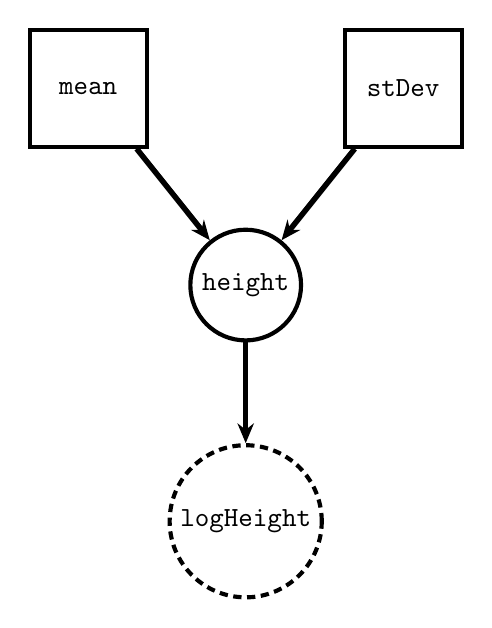
\begin{tikzpicture}
\node [constnode, minimum size=21mm] (mean) at (0,2) {\texttt{mean}};
\node [constnode, minimum size=21mm] (stdev) at (4,2) {\texttt{stDev}};
\node [stochnode, minimum size=12mm] (h) at (2,-0.5) {\texttt{height}}; 
\node [detnode, minimum size=12mm] (logh) at (2,-3.5) {\texttt{logHeight}}; 

\draw[-{Stealth[length=0.25cm, width=0.25cm, angle'=45]}, line width=2pt, color=black] (mean) -- (h);
\draw[-{Stealth[length=0.25cm, width=0.25cm, angle'=45]}, line width=2pt, color=black] (stdev) -- (h);
\draw[-{Stealth[length=0.25cm, width=0.25cm, angle'=45]}, line width=2pt, color=black] (h) -- (logh);
\end{tikzpicture}
\end{figure}

\vspace*{-1cm}

\section*{Vectors}

Before we get to actual Bayesian inference of free model parameters, let's introduce one more piece of Rev syntax: \textit{vectors}. Vectors are containers that contain multiple variables of the same kind. For example, I can have a vector of numbers, or a vector of text strings, but I can't mix numbers and strings in the same vector. Moreover, vectors are ordered: the vectors $[2, 1, 3]$ and $[1, 3, 2]$ are mutually distinct even though they contain the exact same elements, because those elements are differently ordered. \\

\noindent Creating a vector in RevBayes is pretty easy: \\

\indent \texttt{> myVector <- [1, 2, 3]} \\
\indent \texttt{> \# This also works:} \\
\indent \texttt{> myVector <- v(1, 2, 3)} \\

\noindent We can access a specific variable in the vector using brackets, \texttt{[i]}, where \texttt{i} is the position (or \textit{index}) of the variable of interest within the vector: \\

\indent \texttt{> \# Print the first element} \\
\indent \texttt{> myVector[1]} \\
\indent \texttt{\ \ \ 1} \\
\indent \texttt{> \# Re-assign the first element (i.e., overwrite its value)} \\
\indent \texttt{> myVector[1] <- 8} \\

\noindent Rather than specify all the values at once, we can also grow a vector one element at a time: \\

\indent \texttt{> anotherVector[1] <- 3} \\
\indent \texttt{> anotherVector[2] <- 4} \\
\indent \texttt{> anotherVector[3] <- 5} \\

\noindent Of course, for big vectors, this method would be pretty laborious. But we can combine it with the \texttt{for} loops we briefly mentioned above. \\

\hrule
\ \\[1ex]
\textbf{Consider the code below:} \\

\indent \texttt{> for(i in 1:10) \{} \\
\indent \texttt{+\ \ \ \ yetAnotherVector[i] <- 2*i + 3} \\
\indent \texttt{+ \} } \\

\noindent \textbf{2a) What is \texttt{yetAnotherVector} going to look like?} \\

\noindent \textbf{2b) Based on what you learned above, show at least one other way in which you could construct this vector (with the same name and the same values).} \\
\hrule

\noindent And there is no reason to limit ourselves to constant variables: you can fill your vectors with deterministic or stochastic variables, too: \\

\indent \texttt{> for(i in 1:10) \{} \\
\indent \texttt{+\ \ \ \ lastVector[i] {\footnotesize $\sim$} dnNormal(0, 1)} \\
\indent \texttt{+ \}}

\section*{Tips and tricks: what to do if\ldots}

{\large
\begin{enumerate}\bfseries
\item \textbf{I need help?}
\end{enumerate}
}

\noindent \textbf{A:} This is another point of similarity between Rev and \textsf{R}. We can type a question mark followed by the name of any function or probability distribution (or even other Rev language objects that we'll learn about later, such as moves and monitors) to access its documentation. For example, by typing \\

\indent \texttt{> ?dnNormal} \\

\noindent we can learn a lot about the normal distribution and how it's implemented in RevBayes. We find out that the distribution is defined over real numbers and takes two arguments, the first one of which (the mean) can be any real number, while the second (the standard deviation) must be a positive real number. We get the full probability density function (which is simple enough here to fit on a single line), and we learn that we can also call the distribution by its alias \texttt{dnNorm} if we want to save ourselves some typing. \\

{\large
\begin{enumerate}\bfseries
\setcounter{enumi}{1}
\item I want RevBayes to forget the variables I created?
\end{enumerate}
}

\noindent \textbf{A:} It is often good practice to start with a clean slate when you're about to run a new analysis. If you're like me, you will re-use the same variable names in multiple analyses, which carries the risk that you may forget to re-define some of them. In that case, the variables would keep the values they had in your last analysis instead of the values they should have in your current analysis, potentially wreaking havoc on your results. To prevent this from happening, we can make RevBayes forget all the variables we created by ``clearing our workspace'': \\

\indent \texttt{> clear()} \\

\noindent RevBayes also gives you more fine-grained control over your workspace by allowing you to get rid of some variables but not others: \\

\indent \texttt{> clear(randomHumanHeight)} \\

{\large
\begin{enumerate}\bfseries
\setcounter{enumi}{2}
\item I hate RevBayes and I want to quit!
\end{enumerate}
}

\noindent \textbf{A:} Just type \texttt{q()} and hit Enter / Return.

\section*{Parameter estimation: coin flipping}

Equipped with what we learned above, we are ready to start using RevBayes for what it's meant for: Bayesian inference of model parameters. We already learned how to build a model, and how to evaluate the likelihood function $p(D \, | \, \theta)$. However, from Graham's lectures, you know that what we're really after in Bayesian inference is the \textit{posterior distribution}, denoted $p(\theta \, | \, D)$. \\

\noindent We will start with a simple and familiar example. In Lecture 9.1 (``Primer on Likelihood''), we learned about the binomial distribution, which describes the probability of achieving $k$ successes in a sequence of $n$ trials: for example, the probability of ending up with $k$ heads after $n$ coin flips.

\begin{center}
\textcolor{blue}{What follows has been adapted from a RevBayes tutorial developed by Prof. Jeremy M. Brown at the Louisiana State University, who is part of the RevBayes core developer team. Jeremy's slides are freely available and you may find them to be a useful supplement to this tutorial: \\
\url{https://molevolworkshop.github.io/faculty/brown/pdf/Brown\_GraphicalModels\_RevBayes.pdf}}
\end{center}

\noindent Let's re-think this earlier example in light of what we learned above. The binomial distribution is going to be our \textit{model}. It has two \textit{parameters}: the probability of a ``success'' (heads coming up), denoted by $p$, and the number of trials, denoted by $n$. I know how many times I flipped the coin, so $n$ is not a free parameter: rather, it is a constant. What I don't know is whether the coin is fair, or in other words, what is the probability of heads coming up. Therefore, $p$ is a \textit{free parameter}, and we'll have to estimate it. Fortunately, we have the data we need to do so, namely, the following sequence of trial outcomes (coin flips):

\begin{center}
HTTHTTHTTTTHHTTHTHTT
\end{center}

\noindent Since the binomial distribution doesn't care about the order of outcomes, we can condense this information into a single number: the number of successes (heads) $k$. Obviously, $k$ depends on the number of trials $n$ in the sense that I can't have more successes than I have trials (i.e., more heads coming up than the total number of coin flips). More importantly, it also depends on $p$: if $p$ is large, I would expect $k$ to be large also, and vice versa. \\

\noindent At this point, we are almost ready to build our model. There is just one key missing ingredient: the \textit{prior distribution} on the parameter we want to estimate ($p$). In Lecture 11.2 (``Bayes' Rule''), we learned that the prior probability is the probability we attribute to a hypothesis (or a parameter value) before we get to observe any data. To be as objective and unbiased as possible, we often like to assume that before observing our data, we are completely ignorant of what the value of our parameter might be. It can be surprisingly difficult to come up with a probability distribution that represents complete ignorance, but in our simple example, it's fortunately pretty easy. Since $p$ is a probability, its value has to lie somewhere between 0 and 1, and since we have no reason to prefer any particular value over any other value, we will assign the same probability (density) to all values from this range. (If you are interested in the philosophy behind this, look up the \textit{principle of indifference}.) There is a probability distribution that does exactly that: we call it the \textit{uniform distribution}. It can be denoted $U(\!A, B)$, where $A$ is the lower bound of the range of allowed values, and $B$ is its upper bound. Accordingly, in our example, we'll be drawing $p$ from a $U(0, 1)$ prior distribution, and our model looks as follows: \\

\begin{figure}[h]
\centering
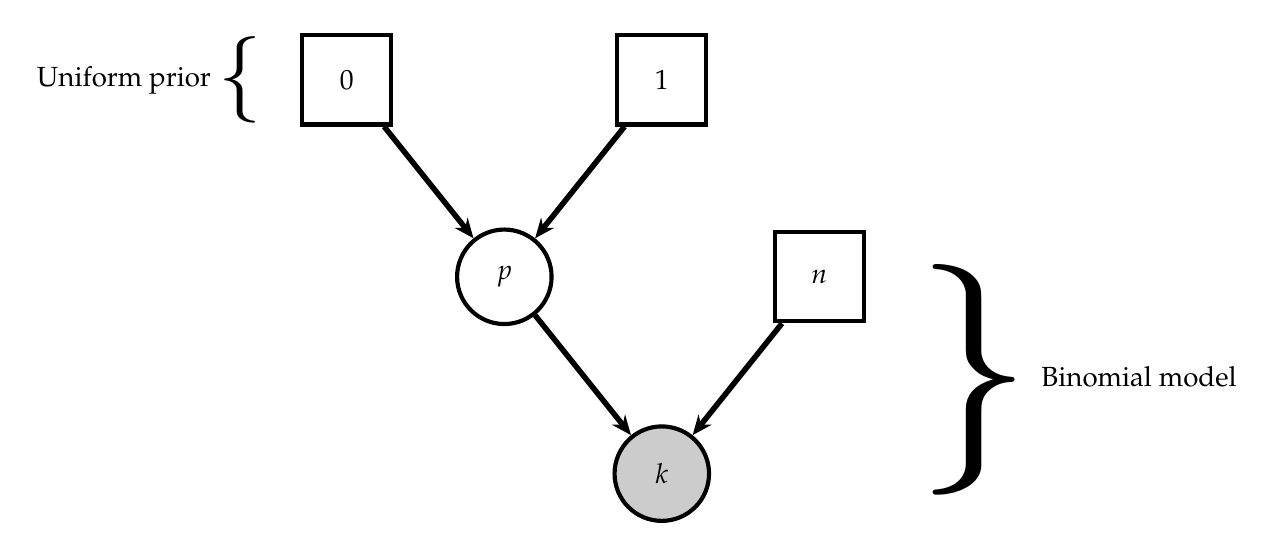
\begin{tikzpicture}
\node [constnode, minimum size=16mm] (min) at (0,2) {0};
\node [constnode, minimum size=16mm] (max) at (4,2) {1};
\node [stochnode, minimum size=12mm] (p) at (2,-0.5) {$p$}; 
\node [constnode, minimum size=16mm] (n) at (6,-0.5) {$n$};
\node [clampnode, minimum size=12mm] (k) at (4,-3) {$k$};
\node (unif) at (-2.5,2) {Uniform prior $\Biggg\{$};
\node (binom) at (9.25,-1.8) {$\Bigggg\}$ Binomial model};

\draw[-{Stealth[length=0.25cm, width=0.25cm, angle'=45]}, line width=2pt, color=black] (min) -- (p);
\draw[-{Stealth[length=0.25cm, width=0.25cm, angle'=45]}, line width=2pt, color=black] (max) -- (p);
\draw[-{Stealth[length=0.25cm, width=0.25cm, angle'=45]}, line width=2pt, color=black] (p) -- (k);
\draw[-{Stealth[length=0.25cm, width=0.25cm, angle'=45]}, line width=2pt, color=black] (n) -- (k);
\end{tikzpicture}
\end{figure}

\hrule
\ \\[1ex]
\textbf{3) How many constant variables are included in this model? How many stochastic variables? How many deterministic ones?} \\
\hrule
\ \\[1ex]
\noindent Let's translate our model into Rev. First, we'll draw the stochastic variable $p$ from its uniform prior: \\

\indent \texttt{p {\footnotesize $\sim$} dnUniform(0, 1)} \\

\noindent Next, we'll create a constant variable for our number of trials (coin flips) $n$: \\

\indent \texttt{n <- 20} \\

\noindent Now we can draw the number of successes (heads) $k$ from the binomial distribution defined by $n$ and $p$: \\

\indent \texttt{k {\footnotesize $\sim$} dnBinomial(n, p)} \\

\noindent While this is a stochastic variable whose possible outcomes can vary, we observed the outcome, and happen to know that the actual number of successes (heads) is 7. So we clamp it to this value: \\

\indent \texttt{k.clamp(7)} \\

\noindent Now we need to tell RevBayes that all of these variables belong to a single model. Since RevBayes is already tracking their relationships for us, we can pick any variable we like, and pass it to the model constructor as a ``handle'': \\

\indent \texttt{myModel = model(k)} \\

\noindent Note that \texttt{myModel} is not a variable: rather, it is an object in my workspace that includes and connects all the previously created variables. We use the equals sign (\texttt{=}) assignment operator to create workspace objects in RevBayes. \\

\noindent Our model is simple enough that we could derive the posterior distribution of $p$ analytically, just like we did with its maximum-likelihood estimate. However, for more complex models -- including those we use in phylogenetics -- this is generally not possible, since the denominator of Bayes' rule quickly devolves into nightmarish multidimensional integrals that make your worst calculus homework look like child's play. As a result, we have to approximate our posterior distribution using numerical methods, the most popular of which is called Markov chain Monte Carlo (MCMC). You'll learn a lot more about it in our next few lectures! \\

\noindent The MCMC algorithm approximates the posterior distribution of $p$ by proposing many different values for it, and evaluating their prior probability as well as likelihood. To do this, we'll have to define some kind of \textit{proposal}, also known as a \textit{move}, that takes the current value of $p$ as its input and returns a new value as its output. Proposals do this by making random draws from some \textit{proposal distribution} centered on the current value. Each parameter that we are estimating needs to have at least one move associated with it. We can store all of our moves in a special vector, which is going to be another one of our workspace objects: \\

\indent \texttt{moves = VectorMoves()} \\

\noindent Right now, this vector is empty, but we can add (or \textit{append}) a move to it. We are going to use the ``slide'' move, which draws new values from a uniform proposal distribution. The \texttt{delta} argument determines the breadth of this distribution, while the \texttt{weight} argument tells RevBayes how often this move should be performed (i.e., how often the value of $p$ should be redrawn): \\

\indent \texttt{moves.append( mvSlide(p, delta=0.1, weight=1) )}

\newpage

\noindent We are almost ready to run our Bayesian analysis! However, as it stands, we have no way to keep track of the parameter values that the analysis is going to sample. We can fix this problem by creating yet another workspace object: a vector of trackers or \textit{monitors}. A monitor can access the current value of the estimated parameter, and -- depending on what kind of monitor we use -- print it either to the screen or to a special log file. Most of the time, we don't actually want to record every single value that the analysis has sampled. (You'll learn why in our forthcoming lectures about MCMC.) Instead, we can tell our monitors to sample, say, only every 100th value: \\

\indent \texttt{monitors = VectorMonitors()} \\
\indent \texttt{monitors.append( mnScreen(printgen=100, p) )} \\
\indent \texttt{monitors.append( mnModel(filename="myMCMC.log", printgen=100, p) )} \\

\noindent Our MCMC analysis consists of our model plus the associated moves and monitors: \\

\indent \texttt{myAnalysis = mcmc(myModel, moves, monitors)} \\

\noindent We created our analysis as yet another workspace object, but haven't run it yet. To do so, we need to run one more line of Rev code: \\

\indent \texttt{myAnalysis.run(20000)} \\

\hrule
\ \\[1ex]
\textbf{4) Refer to lectures (once available) or go with your own best guess: what do you think this `20,000' means?} \\
\hrule
\ \\[1ex]
\noindent If you did everything correctly, you should see something like this in your terminal / command-line window: \\

\begin{center}
\noindent\includegraphics[width=0.8\textwidth]{revbayes-screenlog.png}
\end{center}

\noindent The output file \texttt{myMCMC.log} is now located in your working directory. (If you're not sure exactly where that is, you can ask RevBayes by entering the \texttt{getwd()} command.) Let's open Tracer and drag the file into the left pane of its window: \\

\begin{center}
\noindent\includegraphics[width=0.8\textwidth]{tracer.png}
\end{center}

\noindent In the right pane, I see a plot of the $p$ values sampled over the course of my analysis, which tells me that RevBayes was exploring values ranging from 0.2 to 0.6. In the left pane, I get a numerical summary of these values. The ``ESS'' column gives me the \textit{\ul{e}ffective \ul{s}ample \ul{s}ize} for the parameter in question. I would like this number to be greater than 200 for my results to be reliable. My analysis didn't collect enough samples to reach this threshold, but it's close enough that I can at least take a look at the other column, which reports the \textit{posterior mean} of parameter $p$. This value represents a good summary of the entire posterior distribution, which we can view by selecting the ``Marginal Density'' tab in the right pane of the Tracer window. \\

\hrule
\ \\[1ex]
\textbf{5) What value did you get for the posterior mean of $p$? Compare it to the maximum-likelihood estimate of this parameter that we derived in Lecture 9.1. Do you think the posterior mean represents a good estimate of this parameter? Why or why not?} \\

\noindent \textbf{6) Visualize your posterior distribution by selecting the ``Marginal Density'' tab in Tracer. How many distinct peaks does it have? What do you think this means?} \\

\noindent \textbf{7) Re-run the analysis 4 more times. (You can change the \texttt{filename} argument of the \texttt{mnModel()} monitor to \texttt{myMCMC1.log}, \texttt{myMCMC2.log}, etc. to prevent RevBayes from overwriting your earlier log files.) How big of a difference do you see between the posterior mean values obtained from each run?} \\

\noindent \textbf{8) Load the log files from all 5 runs into Tracer. At the top of the left pane, you should now see a new item called ``Combined'', which represents the pooled sample from all 5 analyses. When you select it, does your new effective sample size exceed 200? What about your posterior mean? Did it get any closer to the maximum-likelihood estimate than the value you reported in question 5)?} \\
\hrule

\end{document}